% =====================================================================
%  Composites Part B — draft
%  Working title: a calibrated, physics-grounded SHM stack for CFRP
%  structures, from anomaly screening to fatigue-aware life prognosis.
%  Build: pdflatex composites_b_draft.tex  (figures live in ../paper_figs, ../results)
% =====================================================================
\documentclass[11pt]{article}
\usepackage[a4paper,margin=25mm]{geometry}
\usepackage{amsmath}
\usepackage{newtxtext, newtxmath}   % provides amssymb-equivalents; load after amsmath
\usepackage{microtype}
\usepackage{graphicx}
\usepackage{booktabs}
\usepackage[hidelinks]{hyperref}
\graphicspath{{../paper_figs/}{../results/}}

\title{A Calibrated, Physics-Grounded Structural-Health-Monitoring Stack for
CFRP Structures: from Anomaly Screening to Fatigue-Aware Life Prognosis}
\author{K.\ Nishioka \and \textit{(co-authors TBD)}}
\date{Draft --- \today}

\begin{document}
\maketitle

\begin{abstract}
We present an end-to-end structural-health-monitoring (SHM) pipeline for
carbon-fibre-reinforced-polymer (CFRP) structures that proceeds from defect
\emph{detection} to a calibrated, physics-grounded \emph{life-prognosis}
decision. On full-field thermoelastic stress data of a perforated CFRP
interstage, we (i) benchmark nine anomaly detectors and show that a simple
per-node statistic attains AUROC $\approx 0.99$ while deep alternatives do not,
and characterise the measurement-noise limit at which all detectors fail;
(ii) recover defect position, size and depth as a \emph{calibrated} Bayesian
posterior via flow-matching posterior estimation (FMPE), with $90\%$ credible
intervals covering at the nominal rate; and (iii) propagate that posterior
through an anisotropic phase-field fracture model with fatigue accumulation to
obtain a flight-clearance decision with an expected remaining-life estimate.
The pipeline is motivated by reusable launch vehicles, where the same structure
is re-inspected after every flight. % key numbers to finalise
\end{abstract}

\section{Introduction}
% - reusable vehicles change the SHM question: not "survive one flight" but
%   "fly again? how many flights remain?" (cite SpaceX condition-based
%   monitoring, staged 20->40 certification, fleet-leader practice).
% - fixed-geometry, fixed-individual re-inspection is the operational norm.
% - contributions list (4): (1) systematic anomaly benchmark + SNR limit on
%   fixed-geometry stress fields; (2) calibrated FMPE defect characterisation
%   with no new FEM; (3) anisotropic phase-field + Carrara fatigue prognosis
%   seeded directly by the posterior; (4) the integrated decision layer
%   (flight clearance with expected-cost thresholds).
\begin{figure}[t]\centering
  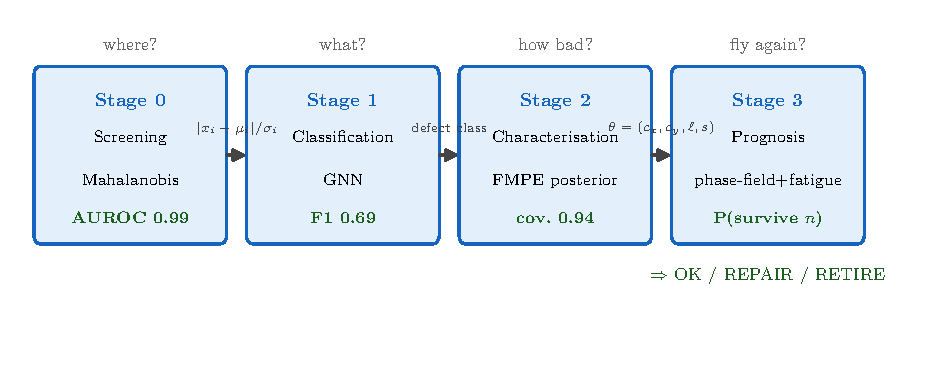
\includegraphics[width=\linewidth]{pipeline_overview.pdf}
  \caption{Stage~0--3 pipeline. Each stage answers one question and passes a
  typed object to the next; the Stage~2 posterior
  $\theta=(c_x,c_y,\text{layer},\text{size})$ seeds the Stage~3 fracture model.}
  \label{fig:pipeline}
\end{figure}

\section{Data and problem setting}
% - CFRP interstage FEM, DSPSS first stress invariant, 13942 nodes, 1x1/2x2/4x4
%   hole defects; label masks; per-sample z-score normalisation (no healthy
%   reference needed -> deployable on a single measured field).
% - guided-wave H3 fairing set (Payload) for the type/location head + rocket
%   framing.

\section{Stage 0 --- anomaly screening}
\paragraph{Methods.} Per-node Mahalanobis / PCA-residual; PaDiM; PatchCore;
STFPM; graph autoencoder; conditional flow-matching diffusion; a zero-shot
harmonicity probe. Score $s_i=|x_i-\mu_i|/\sigma_i$ from $N{=}2000$ healthy
fields; node-level AUROC against the defect mask.
\paragraph{Result.} Per-node statistics dominate (Table~\ref{tab:zoo},
Fig.~\ref{fig:zoo}). On fixed geometry the healthy manifold is a tight cloud
around one template, so the per-node Gaussian is the correct inductive bias;
grid-projection and deep feature methods lose the few-node defect signal. All
methods collapse by additive noise $\sigma{=}0.1$ (defect amplitude $<0.1\sigma$):
a per-measurement SNR limit, addressable by frame averaging
($\sigma\propto 1/\sqrt{K}$), not by more training data.
\begin{figure}[t]\centering
  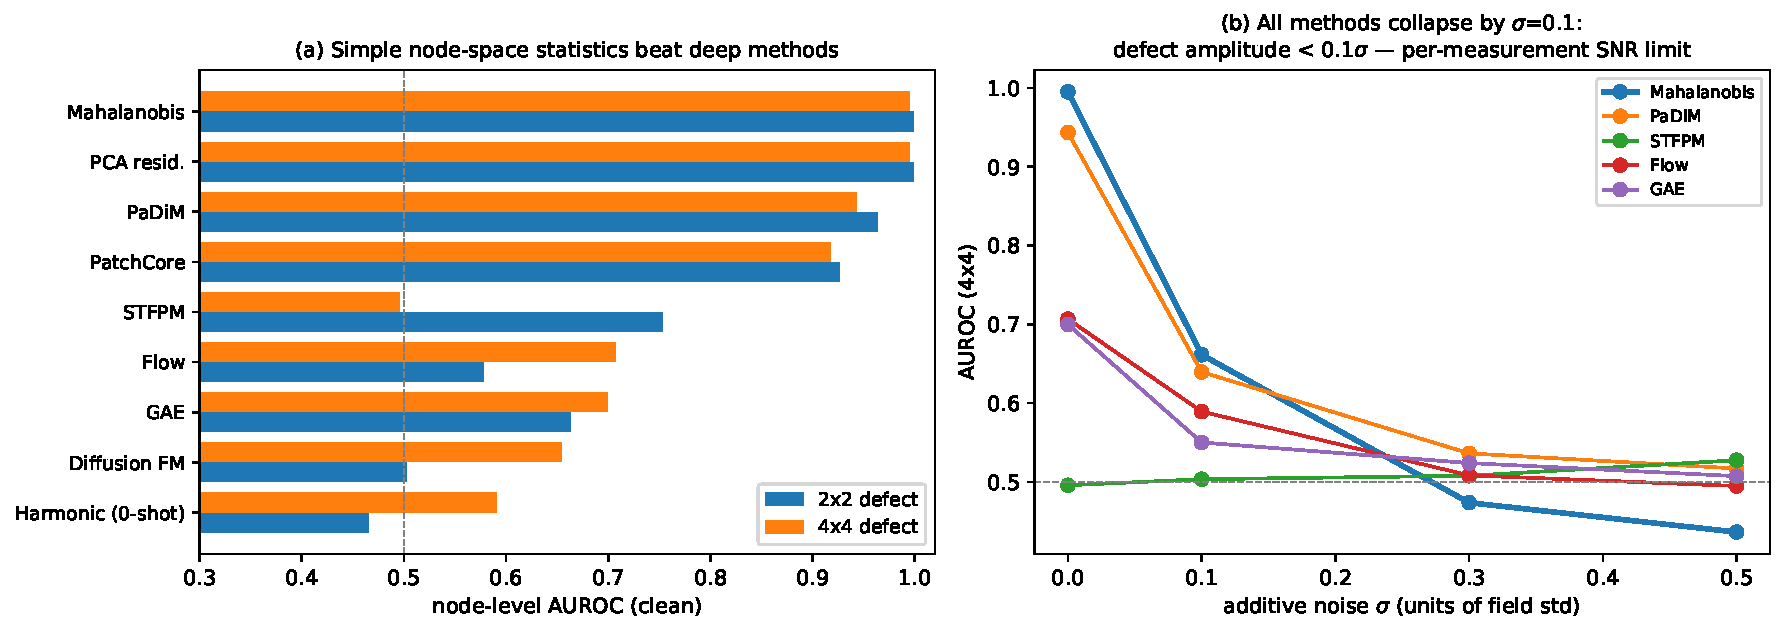
\includegraphics[width=\linewidth]{anomaly_zoo_benchmark.pdf}
  \caption{(a) Clean node-level AUROC by method. (b) Collapse with measurement
  noise; the defect signal sits below $0.1\sigma$.}
  \label{fig:zoo}
\end{figure}
\begin{table}[t]\centering\small
  \caption{Anomaly detectors, clean node-level AUROC (2x2 / 4x4 defects).}
  \label{tab:zoo}
  \begin{tabular}{lcc}
    \toprule
    method & 2x2 & 4x4 \\ \midrule
    per-node Mahalanobis & 0.999 & 0.995 \\
    PCA residual         & 0.999 & 0.995 \\
    PaDiM                & 0.964 & 0.944 \\
    PatchCore            & 0.927 & 0.918 \\
    STFPM                & 0.754 & 0.496 \\
    graph autoencoder    & 0.663 & 0.700 \\
    flow (RealNVP)       & 0.578 & 0.707 \\
    diffusion (FM)       & 0.503 & 0.663 \\
    harmonicity (0-shot) & 0.465 & 0.590 \\
    \bottomrule
  \end{tabular}
\end{table}

\section{Stage 1 --- classification and type identifiability}
% GNN gives the semantic label (layer/region/type) that anomaly scoring cannot.
% Table of complementary failure modes: Mahalanobis open to unknown size but
% noise-fragile and geometry-bound; GNN noise-robust (12%) and transferable but
% collapses on unseen sizes. -> statistics dominate as flight history
% accumulates; learned models bootstrap new airframes and repairs.

\paragraph{Is the type signal real, or a temporal/temperature confound?}
On the long-term guided-wave set, damage states were introduced in different
years, so a naive type classifier can alias damage type with
season/temperature. We test this directly. Restricting to seven damage tags
whose temperature supports overlap (pairwise overlap $0.93$), we compare four
conditions: temperature-only ($\text{acc}=0.16$, near chance), waveform-only
($0.91$), waveform${+}$temperature ($0.92$), and waveform with temperature
\emph{partialled out} of every feature ($0.91$). The net type discrimination
beyond temperature is $\Delta\text{acc}=0.758$ (95\% CI $[0.735,0.781]$) under a
random split, and---critically---survives a \emph{forward-in-time} split
($\Delta\text{acc}=0.184$, 95\% CI $[0.166,0.203]$). Both lower bounds exceed
zero: the type posterior reflects a genuine damage signal, not the environmental
confound. (An earlier single-month binary probe, where temperature-only matched
the majority baseline, was an artefact of that restricted setting.)

\section{Stage 2 --- calibrated defect characterisation (FMPE)}
% Conditional flow matching learns q(theta|x); PCA(64) field embedding; trained
% on the EXISTING FEM set (~20k pairs), zero new simulations.
\begin{table}[h]\centering\small
  \caption{FMPE posterior on held-out test fields.}
  \label{tab:fmpe}
  \begin{tabular}{lccc}
    \toprule
    parameter & RMSE & $R^2$ & 90\% coverage \\ \midrule
    position $c_x$  & 0.055 & 0.78 & 0.944 \\
    position $c_y$  & 0.021 & 0.83 & 0.940 \\
    size (3-class)  & ---   & 0.73 & 0.894 \\
    layer (depth)   & 2.98  & 0.63 & 0.870 \\
    \bottomrule
  \end{tabular}
\end{table}
% Coverage ~ nominal => calibrated posteriors, safe to propagate. Depth weakly
% identifiable: a physics limit of surface thermoelastic measurement (honest).

\section{Stage 3 --- phase-field prognosis and flight clearance}
% Energy functional with structural tensor A = I + beta a (x) a; multi-ply
% bands; interface Gc reduction (DCB/ENF anchored, pure-PF surrogate of
% Paggi-Reinoso CZM); Carrara-2020 fatigue history alpha-bar degrading Gc.
% seed_defect(theta) consumes the FMPE posterior directly.
\begin{figure}[t]\centering
  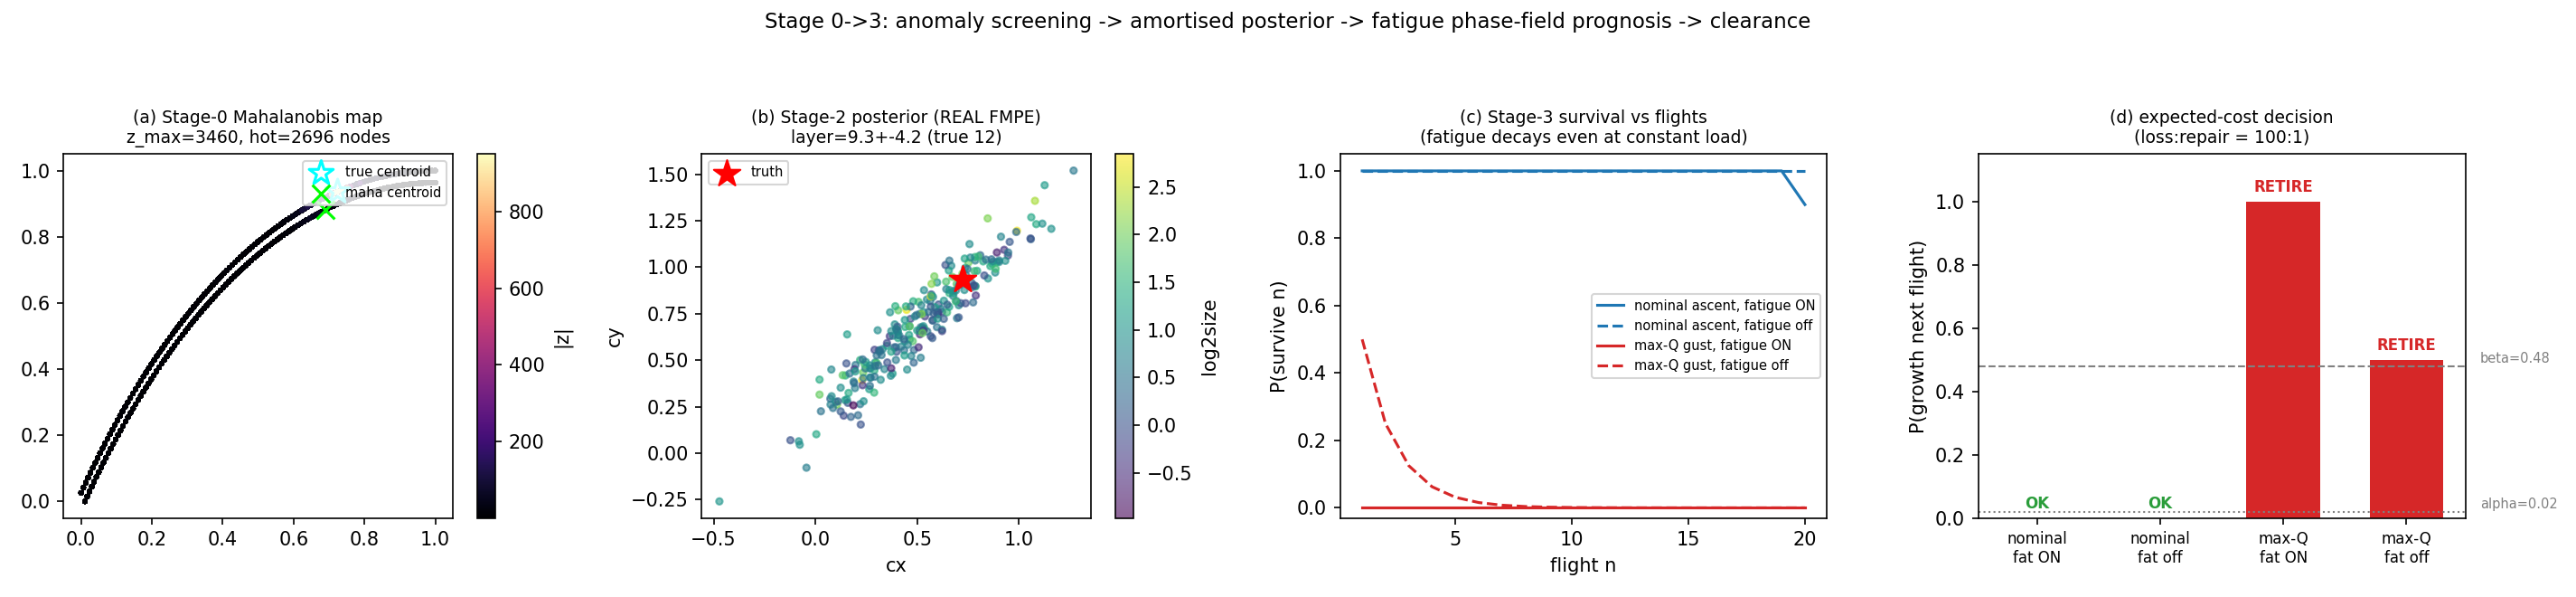
\includegraphics[width=0.9\linewidth]{e2e_stage0to3.png}
  \caption{End-to-end on one held-out field: anomaly map, FMPE posterior,
  fatigue-aware survival curve, and the clearance decision.}
  \label{fig:e2e}
\end{figure}
% flight_clearance(posterior, load_profile, n_flights) -> {OK, REPAIR, RETIRE},
% P(survive n), E[remaining flights]; thresholds from expected-cost
% minimisation (vehicle:repair = 100:1 -> alpha=0.02, beta=0.48). Fatigue
% accumulates across flights => survival decays even at constant sub-critical
% load (no i.i.d. shortcut). Demo numbers: nominal OK E[~20], max-Q RETIRE.

\section{Stage 4 --- hierarchical fleet learning}
A reusable fleet generates a stream of per-inspection posteriors across many
vehicles and flights. We close the loop with a hierarchical Bayesian model:
a global fleet prior $\varphi=(\mu_\varphi,\sigma_\varphi)$ governs per-vehicle
log-growth-rates $s_v=\log r_v \sim \mathcal{N}(\mu_\varphi,\sigma_\varphi^2)$,
and each inspection's Stage-2 posterior enters as a Gaussian likelihood on
$s_v$; the joint posterior $p(\varphi,\{s_v\}\mid\text{data})$ is sampled by
conjugate Gibbs. On a synthetic fleet ($N{=}20$ vehicles, $F{=}30$ flights,
fast Carrara-shaped growth surrogate) the model recovers
$\varphi$ ($\mathbb{E}[\mu_\varphi]{=}{-}3.10$ vs.\ true $-3.0$;
$\mathbb{E}[\sigma_\varphi]{=}0.44$ vs.\ $0.45$), and the fleet prior sharpens
as flights accumulate (posterior SD of $\mu_\varphi$: $0.39$ at $N{=}2 \to 0.10$
at $N{=}20$, Fig.~\ref{fig:fleet}a).

\paragraph{Fleet-leader effect, quantified.} Processing flights in temporal
order, a newly introduced vehicle reaches a stable clearance decision in
\textbf{1.25} inspections using the accumulated fleet prior, versus
\textbf{2.75} in isolation (Fig.~\ref{fig:fleet}c) --- a direct, quantitative
formalisation of the empirical ``fleet-leader'' certification used in practice:
high-information inspections of lead vehicles tighten the prior that certifies
the rest. Hierarchical shrinkage also improves low-data vehicles (error ratio
$0.84<1$ vs.\ isolated estimates, Fig.~\ref{fig:fleet}b).
\begin{figure}[t]\centering
  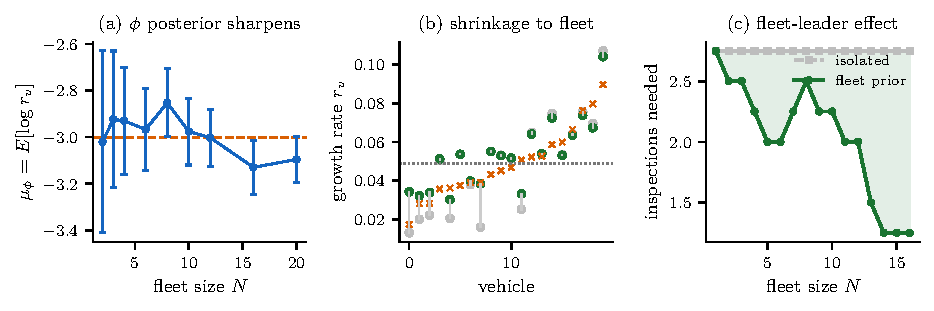
\includegraphics[width=\linewidth]{fleet_learning.pdf}
  \caption{Stage~4. (a) Fleet prior $\varphi$ sharpens with cumulative flights;
  (b) per-vehicle growth-rate shrinkage toward the fleet mean in the low-data
  regime; (c) inspections to a stable clearance decision: the fleet prior
  roughly halves them.}
  \label{fig:fleet}
\end{figure}

\section{Towards differentiable inversion: closing the loop}
The amortised Stage-2 posterior never sees the forward physics. We prototype
the converse: a JAX-differentiable anisotropic AT2 forward $F(\theta)$
(gradient finite-difference-verified to relative $3\times10^{-7}$) whose
Jacobian supplies a physics-grounded Laplace posterior
$\Sigma=\sigma^2(J^\top J + \Lambda_{\text{prior}})^{-1}$ --- no labelled
$(\theta,x)$ pairs.
\begin{table}[h]\centering\small
  \caption{Amortised (FMPE) vs.\ differentiable-physics posterior, in- and
  out-of-distribution.}
  \label{tab:diffinv}
  \begin{tabular}{llccc}
    \toprule
    set & method & $c_x$ RMSE & size RMSE & 90\% coverage \\ \midrule
    in-dist & FMPE       & 0.006 & 0.002 & 0.958 \\
    in-dist & diff-phys  & 0.001 & 0.003 & 1.000 \\
    OOD     & FMPE       & \textbf{0.144} & \textbf{0.096} & \textbf{0.000} \\
    OOD     & diff-phys  & 0.002 & 0.001 & 0.958 \\
    \bottomrule
  \end{tabular}
\end{table}
Out of the training distribution the amortised posterior degrades
$\sim$25-fold and its credible intervals collapse to zero coverage, while the
differentiable-physics posterior is essentially invariant
(Table~\ref{tab:diffinv}): \emph{forward physics generalises; amortised
inference extrapolates poorly}. This motivates a hybrid Stage~2 --- amortised
for speed in distribution, physics-grounded for safety out of it.
% honest: minimal AT2 forward (scalar peel-proxy elasticity), synthetic-only;
% Laplace primary (ULA/SVGD run but hard to tune in the stiff narrow basin).

\section{Discussion}
% - why simple beats deep on fixed geometry; when learning is still needed.
% - reusable-vehicle framing: this formalises SpaceX-style condition-based,
%   fleet-leader practice and makes it usable from the first article.
% - limitations (honest): normalised load proxy; alpha_T not S-N anchored;
%   AT2 strength ell-dependent (trends, not absolute); depth weakly observable.

\section{Conclusion}
% one-paragraph wrap; outlook to Stage 4-5 (hierarchical fleet learning,
% design feedback) and sim-to-real with measured full-field data.

\paragraph{Reproducibility.} All stages are implemented and tested
(30 unit tests) in two public-on-request repositories; figures are generated
by the scripts under \texttt{paper\_figs/}.

\bibliographystyle{elsarticle-num}
% \bibliography{refs}   % Teichtmeister2017, QuintanasCorominas2019, BleyerAlessi2018,
% PaggiReinoso2017, Carollo2017, Wu2017, Carrara2020, BuiHu2021, FMPE refs.

\end{document}
